\section{Relative Position Estimator}

\subsection{System Architecture}
\begin{frame}{\thesection. \insertsection \ - \insertsubsection}
	\begin{figure}
		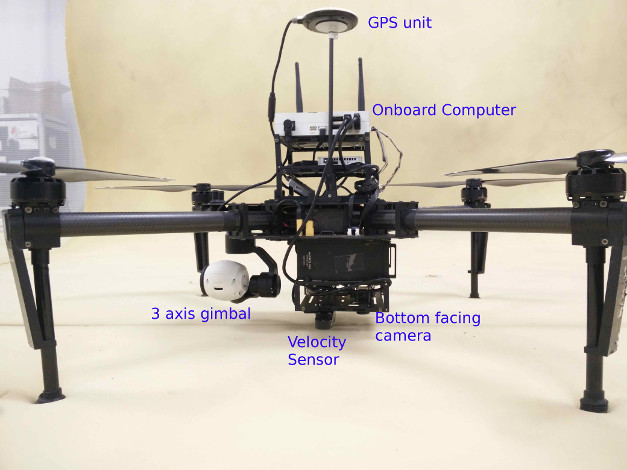
\includegraphics[width=0.6\paperwidth]{figures/m100.jpg}
		\caption{The DJI M100 is equipped with an onboard INS fusing data from
		the GPS, IMU and velocity sensor. We add a 3 axis gimbal and a bottom facing wide angle camera for
		AprilTag detection.}
	\end{figure}
\end{frame}

% ----------------------------------------------------------------------

\begin{frame}{\thesection. \insertsection \ - \insertsubsection}
	\begin{figure}
		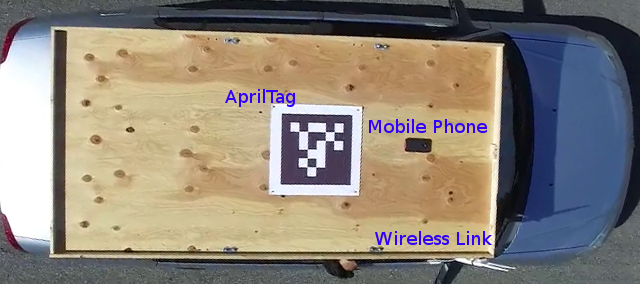
\includegraphics[width=0.8\paperwidth]{figures/car.png}
		\caption{AprilTags allow for 6DoF visual pose estimation by solving a least squares problem
	after extracting the 4 corners of the tag. The mobile phone provides IMU and GPS data.}
	\end{figure}
\end{frame}

% ----------------------------------------------------------------------

\subsection{Kalman Filter}
\begin{frame}{\thesection. \insertsection \ - \insertsubsection}
	\begin{figure}
		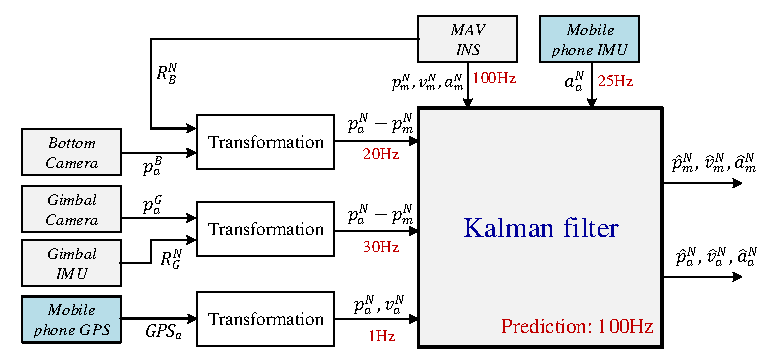
\includegraphics[width=0.85\paperwidth]{figures/kf.pdf}
		\caption{Estimator inputs and outputs. $m$ denotes the MAV frame and $a$ denotes the AprilTag (or car) frame.
		Note that the INS takes care of the MAV's non-linearities for us.}
	\end{figure}
\end{frame}

% ----------------------------------------------------------------------

%\subsection{Kalman Filter}
%\begin{frame}{\thesection. \insertsection \ - \insertsubsection}
%	Process model
%\end{frame}

% ----------------------------------------------------------------------

%\subsection{Kalman Filter}
%\begin{frame}{\thesection. \insertsection \ - \insertsubsection}
%	Measurement model
%\end{frame}

% ----------------------------------------------------------------------